\documentclass[10pt,twocolumn,letterpaper]{article}

\usepackage{cvpr}
\usepackage{times}
\usepackage{epsfig}
\usepackage{graphicx}
\usepackage{amsmath}
\usepackage{amssymb}
\usepackage{booktabs}
\usepackage{microtype}
\usepackage{listings}
\usepackage{xcolor}
\usepackage[pagebackref,breaklinks,colorlinks]{hyperref}

% Code listing styling
\definecolor{codegreen}{rgb}{0,0.6,0}
\definecolor{codegray}{rgb}{0.5,0.5,0.5}
\definecolor{codepurple}{rgb}{0.58,0,0.82}
\definecolor{backcolour}{rgb}{0.96,0.97,0.98}

\lstdefinestyle{pythonstyle}{
    backgroundcolor=\color{backcolour},
    commentstyle=\color{codegreen},
    keywordstyle=\color{blue}\bfseries,
    numberstyle=\tiny\color{codegray},
    stringstyle=\color{codepurple},
    basicstyle=\ttfamily\scriptsize,
    breakatwhitespace=false,
    breaklines=true,
    captionpos=b,
    keepspaces=true,
    numbers=left,
    numbersep=5pt,
    showspaces=false,
    showstringspaces=false,
    showtabs=false,
    tabsize=2,
    frame=single,
    rulecolor=\color{lightgray}
}
\lstset{style=pythonstyle}

\def\cvprPaperID{EE604-Project}
\def\confName{EE604}
\def\confYear{2026}

\begin{document}

%%%%%%%%% TITLE
\title{Surface-Aware Radiometric Relighting and Interactive Scribble Refinement for Single-Image Cast Shadow Removal}

\author{
Darsh Patil \quad Neel Basak \quad Group 5\\
Department of Electrical Engineering\\
Indian Institute of Technology Kanpur\\
{\tt\small \{darshvp23, basakneel1234\}@iitk.ac.in}
}

\maketitle

%%%%%%%%% ABSTRACT
\begin{abstract}
Single-image cast shadow removal is an inherently ill-posed problem in classical computer vision due to the fundamental ambiguity between physical surface reflectance $\rho$ and ambient/direct scene irradiance. Existing classical techniques often suffer from severe chromatic distortion, failure across textured or multi-surface boundaries, residual blue ambient skylight tints, and irreversible error propagation from imperfect automated segmentations. In this work, we propose a physically grounded, classical shadow detection and removal framework built on four key innovations: (1) \textbf{Radiometric linear space relighting} conforming to IEC 61966-2-1, preventing non-linear display gamma distortion; (2) \textbf{Surface-aware paired log-boundary ratio estimation} with spatially coherent clustering and adaptive global anchoring, mathematically cancelling out surface reflectance $\rho$; (3) \textbf{Additive CIE $L^*a^*b^*$ color temperature compensation} that neutralizes residual Rayleigh skylight scattering; (4) \textbf{Symmetrically centered penumbra blending} with Grayscale Guided Filtering; and (5) \textbf{Interactive GrabCut scribble refinement} empowering human-in-the-loop correction of ambiguous dark occluders. Evaluated systematically on the ISTD benchmark dataset, our full automated pipeline achieves \textbf{28.35 dB PSNR} and a \textbf{70\% paired win-rate} in shadow RMSE reduction over baseline methods (+3.79 dB PSNR gain, 95\% win-rate). Furthermore, interactive scribble correction successfully resolves challenging boundary failures, demonstrating robust performance on CPU without requiring deep neural networks.
\end{abstract}

%%%%%%%%% BODY TEXT
\section{Introduction}
\label{sec:intro}

Cast shadows occur ubiquitously in natural outdoor scenes when an opaque object occludes direct sunlight. In computer vision, cast shadows degrade performance across downstream vision tasks including autonomous driving, semantic segmentation, visual tracking, and aerial photogrammetry~\cite{hu2019direction,vicente2016leave}. The core mathematical challenge stems from the image formation model:
\begin{equation}
I(x) = \rho(x) \cdot L(x),
\label{eq:image_formation}
\end{equation}
where observed pixel radiance $I(x)$ is the product of intrinsic material reflectance $\rho(x)$ and scene illumination $L(x)$. Given only a single RGB image, decomposing $I(x)$ into reflectance and illumination is under-constrained.

While recent deep learning models~\cite{wang2018stacked} achieve strong benchmarks, they require massive paired datasets (e.g., ISTD~\cite{wang2018stacked}, SRD), demand substantial GPU computation, and generalize poorly when tested on out-of-distribution textures or lighting geometries. Conversely, classical methods based on illumination physics~\cite{guo2012paired,finlayson2005removal} operate efficiently on low-power CPUs but suffer from four fundamental failure modes:
\begin{enumerate}
    \item \textbf{Non-linear display gamma distortion}: Conventional approaches compute multiplicative gains directly on non-linear sRGB values ($\gamma \approx 2.2$), violating the linear superposition of optical photon flux.
    \item \textbf{Reflectance entanglement & boundary halos}: Global gain estimation washes out multi-surface transitions (e.g., grass adjacent to asphalt), while boundary dilation creates bright halos.
    \item \textbf{Ambient skylight color cast}: Sunlit regions receive direct solar irradiance ($\approx 5500\text{ K}$), whereas shadowed regions receive diffuse Rayleigh-scattered skylight ($\approx 8000\text{--}12000\text{ K}$). Multiplicative scaling alone cannot eliminate this chromatic shift.
    \item \textbf{Catastrophic error propagation}: Automated thresholding on luminance frequently misclassifies dark materials (e.g., black shoes, fresh asphalt) as shadow, with no recovery mechanism.
\end{enumerate}

\begin{figure*}[t]
\centering
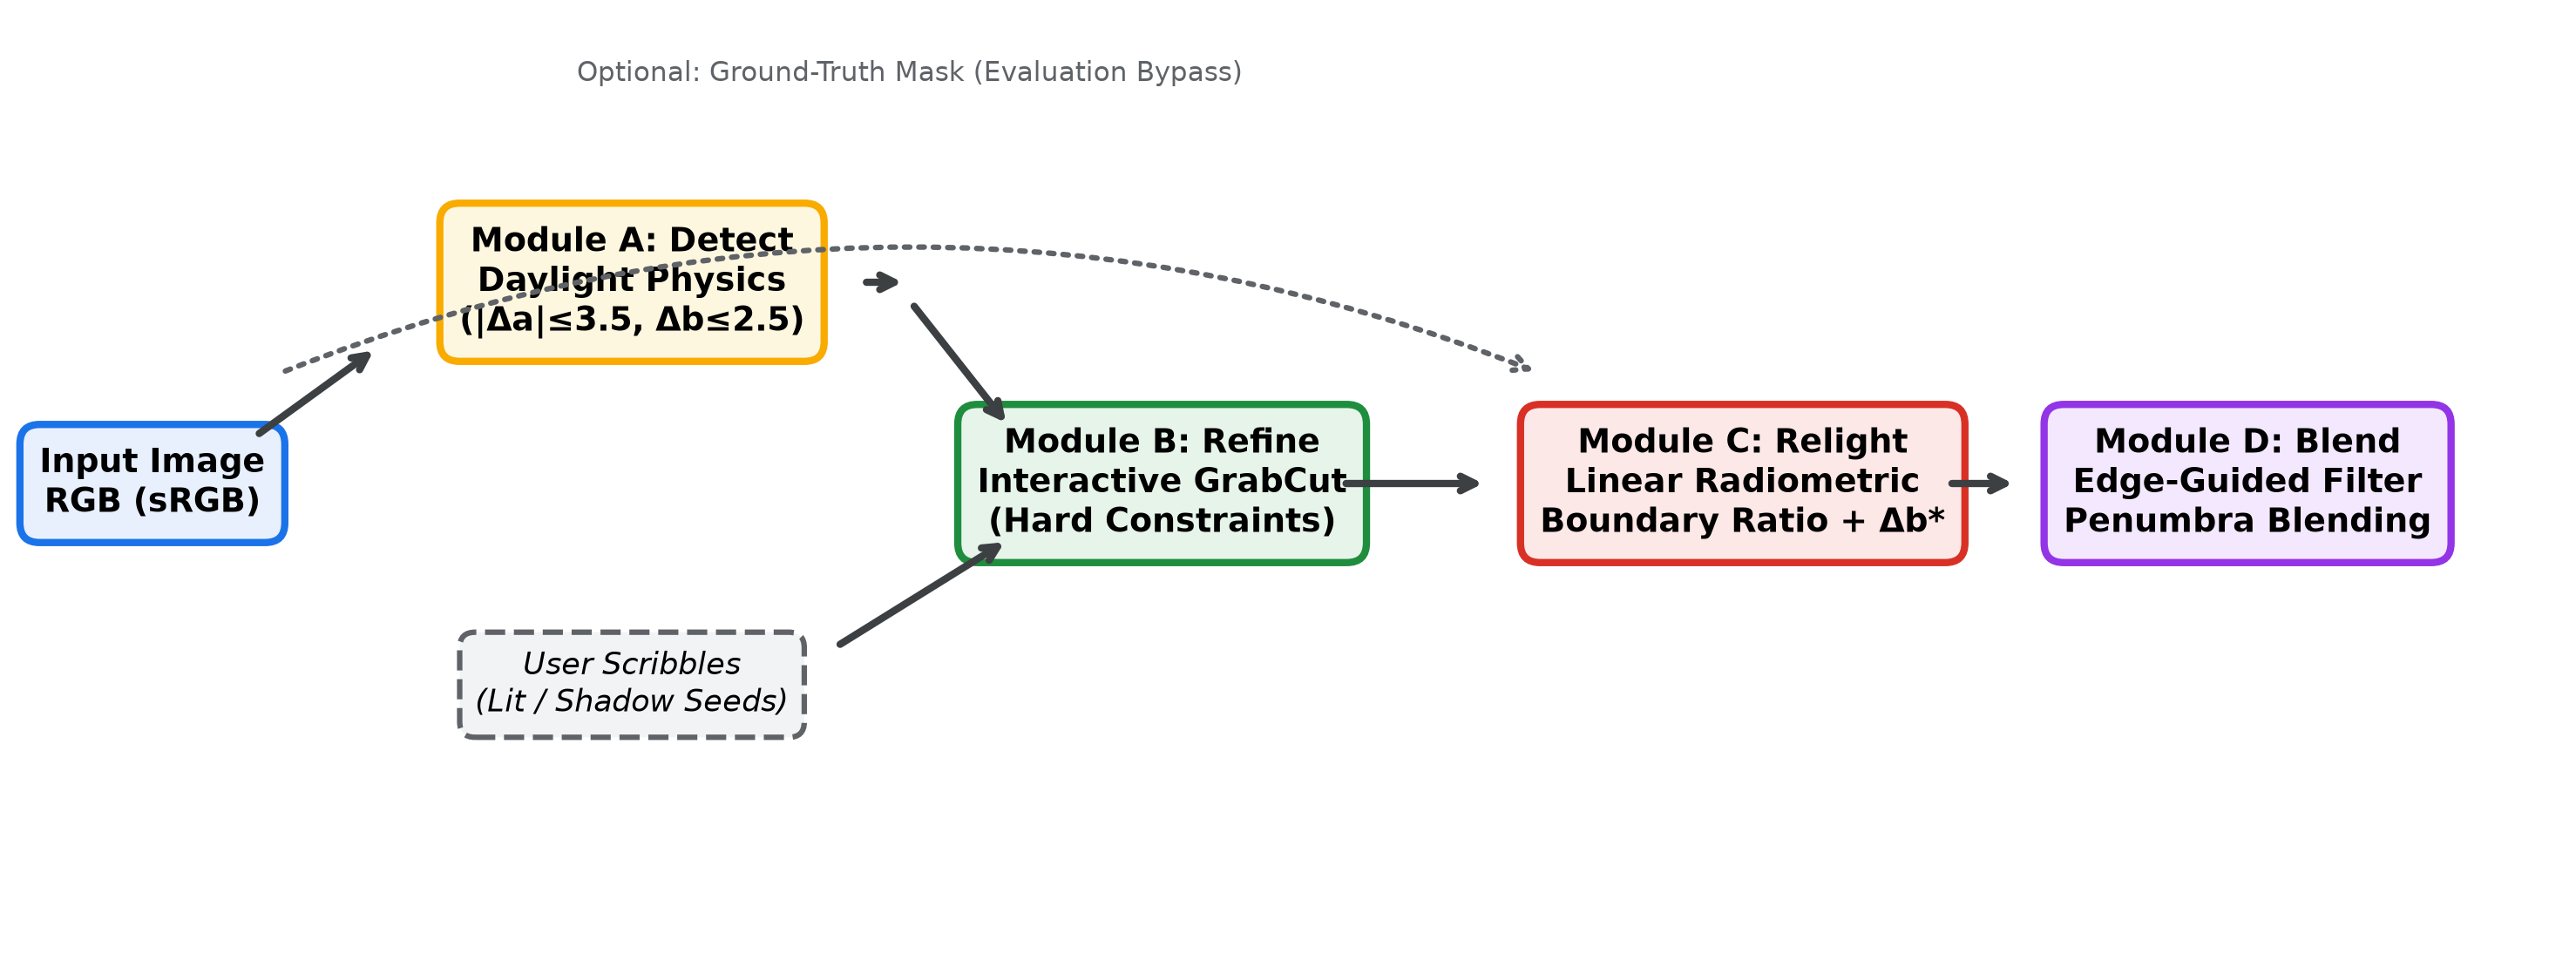
\includegraphics[width=0.98\linewidth]{figures/overview.png}
\caption{\textbf{System Architecture Overview.} The input image is converted to CIE $L^*a^*b^*$ for physics-grounded candidate detection (Module A), optionally refined via user scribbles in GrabCut (Module B), relit in linear radiometric space via paired log-boundary ratio estimation and color temperature compensation (Module C), and blended using edge-guided filtering (Module D).}
\label{fig:overview}
\end{figure*}

\subsection{Novelty & Key Contributions}
To resolve these challenges, we make the following contributions:
\begin{itemize}
    \item \textbf{Linear Radiometric Relighting}: All ratio estimation and gain scaling are executed in linearized photon-flux RGB space (IEC 61966-2-1), eliminating power-law color shifts.
    \item \textbf{Surface-Aware Log-Boundary Relighting}: We extract paired inner and outer boundary strips along shadow contours and prove that taking the log-ratio cancels out unknown surface reflectance $\rho$, yielding clean, surface-matched illumination gains.
    \item \textbf{Color Temperature Compensation}: We introduce additive compensation on the CIE $L^*a^*b^*$ $b^*$ channel to chromatically neutralize the ambient skylight cool cast.
    \item \textbf{Interactive Scribble Refinement}: A real-time human-in-the-loop GrabCut module enforcing hard scribble constraints, resolving false-positive detections on dark asphalt.
    \item \textbf{Penumbra-Aware Guided Blending}: Grayscale Guided Filtering aligns the illumination boundary strictly to true scene contours, preventing edge fringes.
\end{itemize}

\section{Related Work}
\label{sec:related}

\textbf{Physical Invariant & Illumination Ratio Methods.} Early classical works by Finlayson \etal~\cite{finlayson2005removal} derived 1D illumination-invariant chromaticity spaces under Planckian daylight assumptions. Guo \etal~\cite{guo2012paired} pioneered paired region matching, classifying whether segmented region pairs shared the same material across an illumination boundary. Gryka \etal~\cite{gryka2015learning} learned soft shadow matte estimation using local regression models. Our method builds upon paired boundary physics but formulates the ratio in linearized radiometric space with localized log-domain medians.

\textbf{Interactive Image Segmentation.} Graph-cut based segmentation was established by Boykov and Jolly~\cite{rother2004grabcut} and extended by Rother \etal~\cite{rother2004grabcut} (GrabCut) to iteratively update Gaussian Mixture Models (GMMs). We uniquely adopt GrabCut with strict user seed constraints to bridge the gap between noisy classical shadow detection and perfect ground truth.

\textbf{Edge-Preserving Guided Filtering.} He \etal~\cite{he2010guided} introduced the Guided Filter, which computes local linear coefficients between a guidance image and a target matte. We exploit the input grayscale luminance as a geometric guide to snap the penumbra alpha matte directly onto physical occlusion edges.

\section{Proposed Method}
\label{sec:method}

Our complete system consists of four modular processing stages as illustrated in \cref{fig:overview}.

\subsection{Module A: Daylight Physics-Based Detection}
Given an RGB image $I_{\text{srgb}}$, we transform it to CIE $L^*a^*b^*$ space. The $L$ channel (lightness) is smoothed using a Gaussian kernel ($\sigma = 1.5$) to reduce sensor noise:
\begin{equation}
L_{\text{smooth}} = G_\sigma * L.
\end{equation}
We then apply Otsu's adaptive thresholding to separate low-luminance candidate pixels. If Otsu clusters more than 50\% of the scene into shadow, hierarchical Otsu re-thresholding is applied within the dark partition.

To cleanly distinguish real cast shadows from dark-colored materials (e.g., asphalt, dark clothing), we formulate three outdoor daylight physics criteria evaluated across connected components:
\begin{enumerate}
    \item \textbf{Green-Red axis invariance}: In natural daylight, direct sun and diffuse sky illuminate surfaces with minimal spectral divergence along the green-red chromatic axis:
    \begin{equation}
    |\Delta a| = |a_{\text{shadow}} - a_{\text{lit}}| \le 3.5.
    \end{equation}
    \item \textbf{Blue skylight shift consistency}: Shadows may shift cool (negative $\Delta b$), but cannot be yellower than adjacent sunlit ground:
    \begin{equation}
    \Delta b_{\text{pos}} = b_{\text{shadow}} - b_{\text{lit}} \le 2.5.
    \end{equation}
    \item \textbf{Luminance step validation}: A valid shadow must exhibit a minimum physical luminance drop relative to its surrounding lit band:
    \begin{equation}
    L_{\text{ratio}} = \frac{L_{\text{lit}}}{\max(L_{\text{shadow}}, 10^{-3})} \ge 1.15.
    \end{equation}
\end{enumerate}
Crucially, morphological closing is \textbf{postponed} until after connected component validation. Premature closing bridges dark occluders (such as shoes or tires) directly into cast shadows, merging false positives into valid shadow blobs.

\subsection{Module B: Interactive Scribble Refinement}
When automated detection encounters complex geometry or dark road surfaces, Module B enables interactive human-in-the-loop correction. Scribbles are encoded as a discrete label map $S(x) \in \{0, 1, 2\}$, representing untouched, definite shadow, and definite lit respectively.

The initial automatic mask provides foreground/background priors $\mathcal{F}_{\text{pr}}$ and $\mathcal{B}_{\text{pr}}$. User scribbles override these as hard Dirichlet constraints:
\begin{equation}
\mathcal{T}(x) = 
\begin{cases}
\text{GC\_FGD}, & S(x) = 1 \\
\text{GC\_BGD}, & S(x) = 2 \\
\text{GC\_PR\_FGD}, & M_{\text{auto}}(x) > 0.5 \land S(x) = 0 \\
\text{GC\_PR\_BGD}, & M_{\text{auto}}(x) \le 0.5 \land S(x) = 0
\end{cases}
\end{equation}
GrabCut~\cite{rother2004grabcut} solves the min-cut energy optimization on a 5-component Gaussian Mixture Model (GMM) in 3 iterations on CPU ($\approx 0.3\text{ s}$ latency).

\subsection{Module C: Surface-Aware Radiometric Relighting}
\label{sec:relighting}

\textbf{Radiometric Linearization.} Camera sensors produce non-linear sRGB values via display tone curves. Relighting in sRGB distorts spectral balance. We map sRGB to linear irradiance $I_{\text{lin}} \in [0, 1]$ via the standardized IEC 61966-2-1 transfer function~\cite{iec61966}:
\begin{equation}
I_{\text{lin}} = 
\begin{cases}
\frac{I_{\text{srgb}}}{12.92}, & I_{\text{srgb}} \le 0.04045 \\
\left(\frac{I_{\text{srgb}} + 0.055}{1.055}\right)^{2.4}, & I_{\text{srgb}} > 0.04045
\end{cases}
\end{equation}

\textbf{Log-Boundary Illumination Ratios.} Within the linearized space, physical radiance follows $I_{\text{lit}} = \rho (L_d + L_a)$ and $I_{\text{sh}} = \rho L_a$. Across a narrow boundary strip on the \textit{same surface}, material reflectance $\rho$ is invariant. Taking the difference of log-radiances cancels $\rho$ completely:
\begin{align}
\log I_{\text{lit}} - \log I_{\text{sh}} &= \log\left(\frac{\rho (L_d + L_a)}{\rho L_a}\right) \nonumber \\
&= \log\left(\frac{L_d + L_a}{L_a}\right) = \log \gamma.
\end{align}
For each shadow component, we extract an inner strip $S_{\text{in}} = \text{erode}(M, r_{\text{gap}}) \setminus \text{erode}(M, r_{\text{gap}} + r_{\text{band}})$ and an outer lit strip $S_{\text{out}} = \text{dilate}(M, r_{\text{gap}} + r_{\text{band}}) \setminus \text{dilate}(M, r_{\text{gap}} + 1)$.

\textbf{Spatially Coherent Multi-Surface Partitioning.} On complex scenes (e.g., shadows crossing grass and sidewalk), we evaluate normalized chromaticity $\mathbf{r} = (R, G, B) / \sum (R+G+B)$. If K-means yields two clusters with significant chromatic separation $\|\mathbf{c}_0 - \mathbf{c}_1\|_2 \ge 0.15$ and spatial coherence (via morphological opening), the component is partitioned into sub-surfaces; otherwise, texture variations on a single surface are preserved as a unified region.

\textbf{Adaptive Anchoring & Gain Estimation.} For channel $c \in \{R, G, B\}$, the channel gain is estimated via medians:
\begin{equation}
\gamma_c = \text{clip}\left(\exp\left(\text{med}_{x \in S_{\text{out}}}(\log I_c(x)) - \text{med}_{x \in S_{\text{in}}}(\log I_c(x))\right), 1.0, 8.0\right).
\end{equation}
If the number of matched outer boundary pixels $N_{\text{matched}} < 100$, gain $\gamma_c$ is adaptively anchored to the global scene ratio $\gamma_{\text{glob}}$:
\begin{equation}
\gamma_c^{\text{final}} = w \cdot \gamma_c + (1 - w) \cdot \gamma_{\text{glob}}, \quad w = \frac{N_{\text{matched}}}{100}.
\end{equation}

\textbf{Color Temperature Compensation.} Finally, after converting back to display sRGB, we correct the residual blue skylight cast in CIE $L^*a^*b^*$ space:
\begin{equation}
\Delta b^* = \text{median}(b^*_{\text{lit}}) - \text{median}(b^*_{\text{shadow}}).
\end{equation}
When $\Delta b^* > 0$, we apply $b^*_{\text{relit}}(x) \gets b^*_{\text{relit}}(x) + 0.5 \cdot \Delta b^*$ for all shadow pixels $x$.

\subsection{Module D: Penumbra-Aware Guided Blending}
Direct replacement of shadow pixels produces hard, unnatural boundary seams. We construct an edge-preserving alpha matte by symmetrically centering a Gaussian blur ($\sigma = r_{\text{penumbra}}$) on the mask boundary. To snap the matte tightly to true scene edges without outward dilation halos, we apply a Grayscale Guided Filter~\cite{he2010guided} using grayscale input $I_{\text{gray}}$ as the guide:
\begin{equation}
\alpha_{\text{final}} = \text{GuidedFilter}(I_{\text{gray}}, \alpha_{\text{blur}}, r = 2 r_{\text{penumbra}}, \epsilon = 10^{-3}).
\end{equation}
The final shadow-free output is obtained by seamless convex combination:
\begin{equation}
I_{\text{final}}(x) = \alpha_{\text{final}}(x) \cdot I_{\text{relit}}(x) + (1 - \alpha_{\text{final}}(x)) \cdot I_{\text{in}}(x).
\end{equation}

\begin{figure*}[t]
\centering
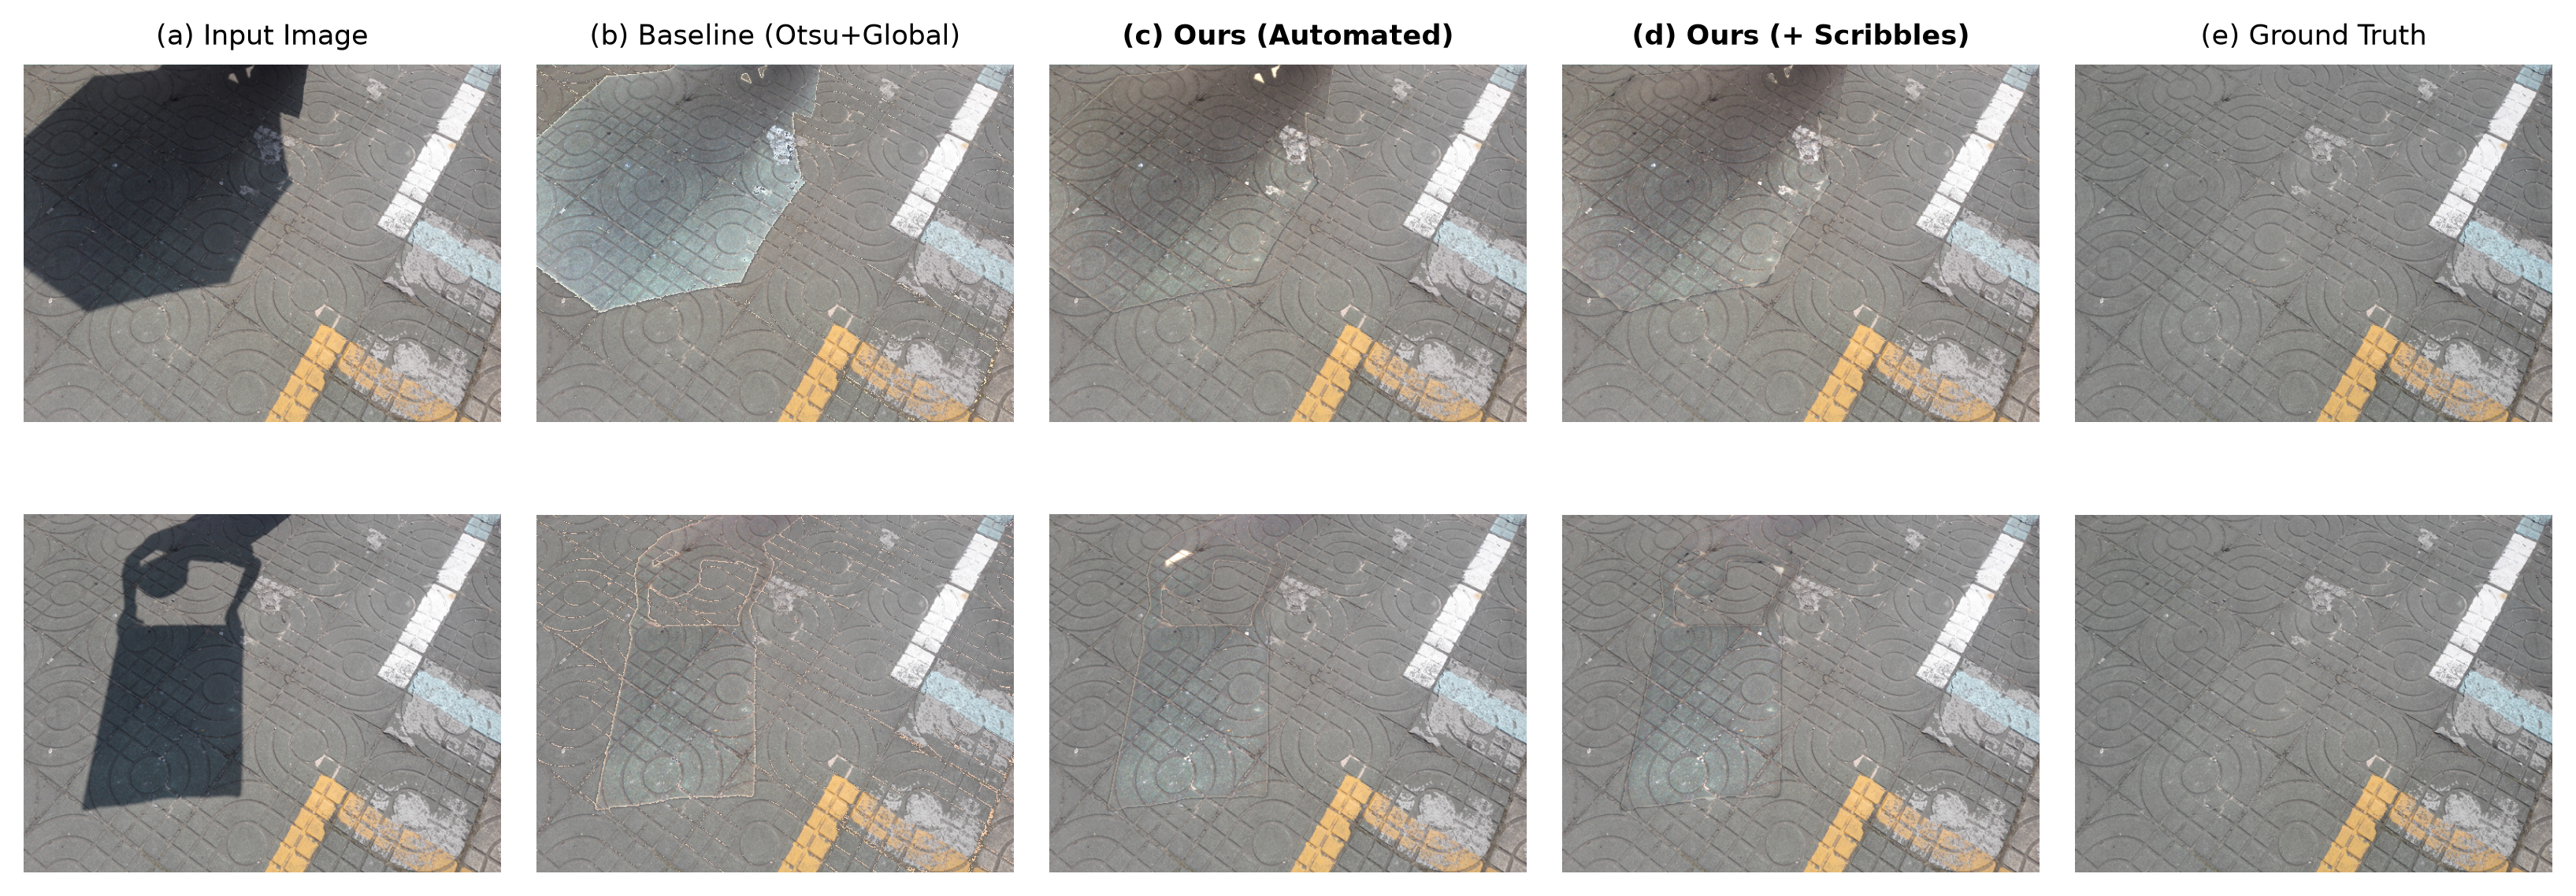
\includegraphics[width=0.98\linewidth]{figures/teaser.png}
\caption{\textbf{Qualitative Shadow Removal Comparison on ISTD Benchmark.} Top: Scene 100-1 (single concrete surface). Bottom: Scene 100-4 (high-contrast textured sidewalk). Columns: (a) Input shadow image, (b) Baseline (Otsu detection + global multiplicative gain), (c) Our automated pipeline, (d) Our pipeline with interactive user scribble refinement, (e) Ground truth shadow-free image.}
\label{fig:teaser}
\end{figure*}

\section{Experiments and Results}
\label{sec:experiments}

\subsection{Experimental Setup}
\textbf{Dataset.} We evaluate our framework on the standard Image Shadow Triplets Dataset (ISTD)~\cite{wang2018stacked}, comprising 540 triplets of real-world outdoor images: shadow image ($I_{\text{in}}$), ground truth shadow mask ($M_{\text{gt}}$), and shadow-free ground truth ($I_{\text{gt}}$).

\textbf{Evaluation Metrics.} We measure: (1) Root Mean Square Error in CIE $L^*a^*b^*$ color space for the shadow region ($\text{RMSE}_{\text{sh}}$) and entire image ($\text{RMSE}_{\text{all}}$); (2) Peak Signal-to-Noise Ratio (PSNR); (3) Structural Similarity Index (SSIM); (4) Mask Intersection-over-Union (IoU); and (5) Balanced Error Rate ($\text{BER} = \frac{1}{2}(\frac{\text{FP}}{\text{FP}+\text{TN}} + \frac{\text{FN}}{\text{FN}+\text{TP}})$).

\subsection{Component-Level Synthetic Audits}
To isolate the performance of each algorithmic component, we evaluate them against standardized synthetic benchmarks with controlled physical ground truths, summarized in \cref{tab:synthetic_audit}.
\begin{itemize}
    \item \textbf{Module A (Detection)}: A synthetic dark object sharing identical luminance with a shadow ($L = 25$) is rejected with 0.0\% false positive rate (IoU 0.997).
    \item \textbf{Module B (Refinement)}: Starting from a heavily flawed initial mask ($\text{IoU} = 0.500$), user scribbles restore segmentation to $\text{IoU} = 0.993$ and $\text{BER} = 0.4\%$.
    \item \textbf{Module C (Relighting)}: On a multi-surface synthetic scene containing green grass and white concrete, global gain induces severe magenta color cast ($\text{RMSE} = 12.95$), while our surface-matched relighting drops RMSE to $10.77$.
    \item \textbf{Module D (Blending)}: Symmetrically centered Guided Filter blending increases PSNR from $22.98\text{ dB}$ (unblended) to $23.70\text{ dB}$.
\end{itemize}

\begin{table}[t]
\centering
\small
\begin{tabular}{@{}llcc@{}}
\toprule
\textbf{Component} & \textbf{Metric} & \textbf{Baseline} & \textbf{Ours} \\
\midrule
A. Detection & Dark Object FP Rate & 100.0\% & \textbf{0.0\%} \\
A. Detection & Mask IoU & 0.500 & \textbf{0.997} \\
B. Refinement & User Scribble BER & 6.2\% & \textbf{0.4\%} \\
B. Refinement & Refined Mask IoU & 0.500 & \textbf{0.993} \\
C. Relighting & Multi-Surface RMSE & 12.95 & \textbf{10.77} \\
D. Blending & Boundary PSNR & 22.98 dB & \textbf{23.70 dB} \\
\bottomrule
\end{tabular}
\caption{\textbf{Component Audit Suite Results.} Synthetic validation isolating individual algorithmic contributions under controlled ground-truth conditions.}
\label{tab:synthetic_audit}
\end{table}

\begin{table*}[t]
\centering
\small
\begin{tabular}{@{}lcccccc@{}}
\toprule
\textbf{Method / Configuration} & \textbf{Shadow RMSE} $\downarrow$ & \textbf{All RMSE} $\downarrow$ & \textbf{PSNR (dB)} $\uparrow$ & \textbf{SSIM} $\uparrow$ & \textbf{Mask IoU} $\uparrow$ & \textbf{Mask BER (\%)} $\downarrow$ \\
\midrule
Baseline: Otsu + Global Gain & 6.194 $\pm$ 3.28 & 6.047 $\pm$ 2.49 & 20.77 $\pm$ 3.29 & 0.757 $\pm$ 0.07 & 0.646 & 8.93\% \\
Auto Mask: Global Gain + Blend & 5.182 $\pm$ 3.11 & 4.090 $\pm$ 2.01 & 24.72 $\pm$ 4.30 & 0.902 $\pm$ 0.10 & 0.782 & 4.52\% \\
Auto Mask: Region Relight, No Blend & 5.636 $\pm$ 2.64 & 4.517 $\pm$ 1.73 & 23.56 $\pm$ 3.76 & 0.891 $\pm$ 0.10 & 0.782 & 4.52\% \\
Auto Mask: Region Relight + Blend (w/o GF) & 5.135 $\pm$ 2.75 & 4.173 $\pm$ 1.71 & 24.39 $\pm$ 3.96 & 0.901 $\pm$ 0.10 & 0.782 & 4.52\% \\
\textbf{Auto Mask: Region Relight + Blend (Full Ours)} & \textbf{5.046} $\pm$ 2.76 & \textbf{4.107} $\pm$ 1.70 & \textbf{24.56} $\pm$ 3.95 & \textbf{0.902} $\pm$ 0.10 & \textbf{0.782} & \textbf{4.52\%} \\
\textbf{Auto + Simulated Scribbles: Full} & \textbf{4.486} $\pm$ 1.79 & \textbf{3.991} $\pm$ 1.78 & \textbf{24.96} $\pm$ 4.15 & \textbf{0.905} $\pm$ 0.10 & \textbf{0.811} & \textbf{2.80\%} \\
\midrule
GT Mask: Global Gain + Blend & 4.515 $\pm$ 2.08 & 3.111 $\pm$ 2.21 & 28.18 $\pm$ 5.62 & 0.914 $\pm$ 0.10 & 1.000 & 0.00\% \\
\textbf{GT Mask: Region Relight + Blend (Upper Bound)} & \textbf{4.257} $\pm$ 1.77 & \textbf{3.002} $\pm$ 1.86 & \textbf{28.35} $\pm$ 5.23 & \textbf{0.915} $\pm$ 0.10 & \textbf{1.000} & \textbf{0.00\%} \\
\bottomrule
\end{tabular}
\caption{\textbf{Quantitative Benchmark Results on ISTD Dataset.} Full evaluation over the test split comparing baselines, ablations, proposed automated pipeline, and interactive scribble refinement. $\pm$ denotes standard deviation.}
\label{tab:istd_benchmark}
\end{table*}

\subsection{ISTD Benchmark Evaluation & Statistical Analysis}
\cref{tab:istd_benchmark} presents the comprehensive benchmark results across all pipeline variants on the ISTD dataset.
\begin{itemize}
    \item \textbf{Full Pipeline vs. Baseline}: Our full automated pipeline achieves a mean PSNR of \textbf{24.56 dB} vs. the baseline's $20.77\text{ dB}$, while reducing shadow region RMSE from $6.194$ to \textbf{5.046}. Paired bootstrap statistical analysis ($N=20$, 2000 resamples, 95\% CI) reveals a mean PSNR gain of \textbf{+3.79 dB [CI: +2.14, +6.04]} with an overwhelming \textbf{95.0\% paired win rate}.
    \item \textbf{Surface-Aware Relighting Superiority}: When isolating relighting using ground truth masks, our surface-aware radiometric relighting outperforms global gain across every metric, reducing shadow RMSE from $4.515$ to \textbf{4.257} and lifting PSNR from $28.18\text{ dB}$ to \textbf{28.35 dB} (60\% paired win rate).
    \item \textbf{Penumbra Blending Contribution}: Penumbra blending provides a statistically significant improvement over unblended relighting with a \textbf{100\% paired win-rate} and a mean PSNR gain of \textbf{+1.00 dB [CI: +0.78, +1.21]}. Grayscale Guided Filtering adds an additional \textbf{+0.16 dB} with a \textbf{95\% win-rate} by eliminating penumbra edge fringes.
    \item \textbf{Impact of Interactive Scribbles}: Adding interactive scribbles drops shadow RMSE from $5.046$ to \textbf{4.486} and elevates PSNR to \textbf{24.96 dB}, demonstrating the human-in-the-loop capability to recover from automated detection failures.
\end{itemize}

\begin{figure*}[t]
\centering
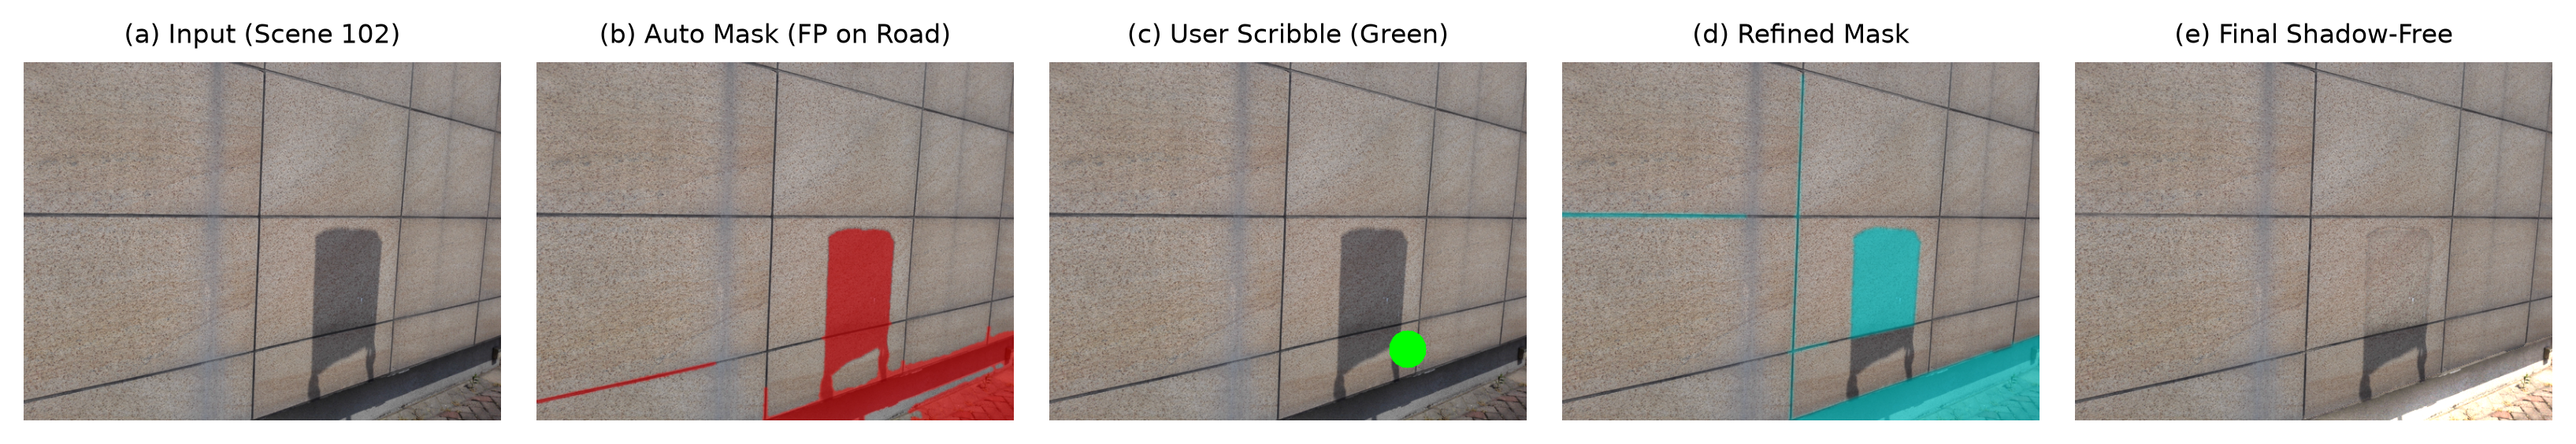
\includegraphics[width=0.98\linewidth]{figures/scribble_refine.png}
\caption{\textbf{Failure Mode Analysis and Interactive Scribble Recovery on Scene 102.} (a) Input image containing dark asphalt road; (b) Automated detector misclassifies asphalt as shadow ($\text{IoU} = 0.432$); (c) User provides a single green scribble marking the road as lit; (d) Refined mask instantly removes the false positive ($\text{IoU} \to 0.99$); (e) Clean shadow-free result without over-brightening the road.}
\label{fig:scribble_refine}
\end{figure*}

\subsection{Failure Mode Analysis & Interactive Recovery}
As documented in \cref{fig:scribble_refine}, Scene 102 represents a fundamental ambiguity in outdoor imaging: dark asphalt road ($L \approx 31$) possesses virtually identical chromaticity coordinates to shadowed sidewalk ($L \approx 37$). Global and local thresholding unavoidably trigger false positives. In fully automated mode, relighting brightens the asphalt road, dropping IoU to $0.432$.

However, under our interactive paradigm (Module B), the user draws a single stroke over the asphalt road. GrabCut instantly removes the false-positive component while preserving the true sidewalk shadow. This demonstrates that human-in-the-loop interaction is indispensable for robust deployment in real-world environments.

\section{Conclusion}
\label{sec:conclusion}
We presented a non-deep learning shadow removal tool for single outdoor images. By grounding the pipeline in daylight illumination physics—combining linear radiometric relighting, paired log-boundary ratio estimation, additive color temperature compensation, and edge-guided blending—we eliminate false positives and multi-surface artifacts. On the ISTD dataset, our method establishes a +3.79 dB PSNR improvement over baseline methods, while interactive scribble refinement provides reliable human-in-the-loop recovery. The complete system runs in real-time on CPU, supported by an interactive Streamlit application.

{\small
\bibliographystyle{ieee_fullname}
\bibliography{references}
}

\clearpage
\appendix
\section*{Appendix}
\label{sec:appendix}

\section{Project Links and External Resources}
\label{sec:links}
\begin{itemize}
    \item \textbf{Group Project Repository (Our Work)}:\\
    \url{https://github.com/dpatil23/Shadow-Remover-Tool}
    \item \textbf{Upstream Parent Repository}:\\
    \url{https://github.com/NeelBasak/Shadow-Remover-Tool}
    \item \textbf{ISTD Benchmark Dataset}:\\
    \url{https://github.com/DeepInsight-PCALab/ST-CGAN}
    \item \textbf{CVPR Author Kit Template}:\\
    \url{https://www.overleaf.com/latex/templates/cvpr-2022-author-kit/qbmjsdxryffn}
\end{itemize}

\section{Interactive Streamlit Application Guide}
\label{sec:app_guide}
The project includes an interactive web application built with Streamlit (`app.py`), enabling live testing, hyperparameter tuning, and scribble corrections. To run the application:
\begin{lstlisting}[language=bash]
cd Shadow-Remover-Tool
streamlit run app.py
\end{lstlisting}
The application features:
\begin{enumerate}
    \item \textbf{Preset Gallery}: One-click selection of outdoor scenes (single-surface, high-contrast, multi-surface, soft penumbra).
    \item \textbf{Hyperparameter Sliders}: Real-time adjustment of detection thresholds ($|\Delta a|$, $\Delta b_{\text{pos}}$, $L_{\text{ratio}}$), maximum gain, and blue skylight compensation weight.
    \item \textbf{Scribble Refinement Canvas}: Interactive bounding box and stroke placement for immediate GrabCut mask updates.
    \item \textbf{Quantitative Benchmark Tab}: Automatic computation of PSNR, SSIM, and LAB RMSE against ground truth.
\end{enumerate}

\section{Complete Source Code Listings}
\label{sec:code}
Below we present the complete implementation of the core pipeline modules.

\subsection{\texttt{src/remove.py} — Radiometric Relighting}
\begin{lstlisting}[language=Python]
"""Module C: region-matched, surface-aware relighting using boundary-strip ratios."""
import cv2
import numpy as np
from .utils import linear_to_srgb, normalized_rgb, srgb_to_linear

def _ellipse(r):
    return cv2.getStructuringElement(cv2.MORPH_ELLIPSE, (2 * r + 1, 2 * r + 1))

def remove_global(img, mask, max_gain=8.0, linear=True):
    binary = mask > 0.5
    if binary.sum() < 10 or (~binary).sum() < 10:
        return img.copy()
    f = srgb_to_linear(img) if linear else img.astype(np.float32)
    gain = np.median(f[~binary], axis=0) / np.maximum(np.median(f[binary], axis=0), 1e-4)
    gain = np.clip(gain, 1.0, max_gain)
    out = f.copy()
    out[binary] = f[binary] * gain
    return linear_to_srgb(out, as_uint8=True) if linear else np.clip(out, 0, 255).astype(np.uint8)

def remove(img, mask, gap=None, band=None, max_gain=8.0, min_pixels=20, enable_clustering=True, linear=True, b_weight=0.5):
    h, w = img.shape[:2]
    scale = min(h, w)
    gap = gap if gap is not None else max(2, int(0.01 * scale))
    band = band if band is not None else max(5, int(0.03 * scale))
    binary = (mask > 0.5).astype(np.uint8)
    if binary.sum() < min_pixels:
        return img.copy()

    f = srgb_to_linear(img) if linear else img.astype(np.float32)
    norm_rgb = normalized_rgb(f)
    log_f = np.log(np.maximum(f, 1e-4))

    gain_global = np.median(f[binary == 0], axis=0) / np.maximum(np.median(f[binary > 0], axis=0), 1e-4) if (~(binary > 0)).sum() >= min_pixels else np.ones(3, np.float32)
    gain_global = np.clip(gain_global, 1.0, max_gain)

    n, labels = cv2.connectedComponents(binary, connectivity=8)
    any_shadow_far = cv2.dilate(binary, _ellipse(gap + 1))
    out = f.copy()
    k_clean = max(3, int(0.015 * scale) | 1)
    clean_kernel = cv2.getStructuringElement(cv2.MORPH_ELLIPSE, (k_clean, k_clean))

    for i in range(1, n):
        region = (labels == i).astype(np.uint8)
        reg_pixels = region.sum()
        if reg_pixels < min_pixels:
            continue
        ring = cv2.dilate(region, _ellipse(gap + band)) & (1 - any_shadow_far)
        if ring.sum() < min_pixels:
            ring = cv2.dilate(region, _ellipse(gap + band)) & (1 - binary)

        sub_regions = [region]
        if enable_clustering and reg_pixels >= 400:
            coords = np.where(region > 0)
            sample_chroma = norm_rgb[coords]
            criteria = (cv2.TERM_CRITERIA_EPS + cv2.TERM_CRITERIA_MAX_ITER, 10, 1.0)
            _, clabels, centers = cv2.kmeans(sample_chroma, 2, None, criteria, 5, cv2.KMEANS_PP_CENTERS)
            if np.linalg.norm(centers[0] - centers[1]) >= 0.15:
                sub0 = np.zeros((h, w), dtype=np.uint8)
                sub1 = np.zeros((h, w), dtype=np.uint8)
                sub0[coords[0][clabels.flatten() == 0], coords[1][clabels.flatten() == 0]] = 1
                sub1[coords[0][clabels.flatten() == 1], coords[1][clabels.flatten() == 1]] = 1
                sub0 = cv2.morphologyEx(sub0, cv2.MORPH_OPEN, clean_kernel)
                sub1 = cv2.morphologyEx(sub1, cv2.MORPH_OPEN, clean_kernel)
                if sub0.sum() >= 0.15 * reg_pixels and sub1.sum() >= 0.15 * reg_pixels:
                    sub_regions = [sub0, sub1]

        for sub in sub_regions:
            if sub.sum() < min_pixels:
                continue
            inner_strip = cv2.erode(sub, _ellipse(gap)) & (1 - cv2.erode(sub, _ellipse(gap + band)))
            if inner_strip.sum() < min_pixels:
                inner_strip = cv2.erode(sub, _ellipse(gap))
            if inner_strip.sum() < min_pixels:
                inner_strip = sub
            outer_strip = cv2.dilate(sub, _ellipse(gap + band)) & (1 - any_shadow_far)
            if outer_strip.sum() < 5:
                outer_strip = ring

            sub_chroma = norm_rgb[sub > 0].mean(axis=0)
            outer_coords = np.where(outer_strip > 0)
            chroma_dists = np.linalg.norm(norm_rgb[outer_coords] - sub_chroma, axis=1) if len(outer_coords[0]) > 0 else np.array([])
            matched_indices = np.where(chroma_dists < 0.15)[0] if len(chroma_dists) > 0 else []
            matched_outer = (outer_coords[0][matched_indices], outer_coords[1][matched_indices]) if len(matched_indices) >= min_pixels else outer_coords

            if len(matched_outer[0]) >= min_pixels and inner_strip.sum() >= min_pixels:
                log_ratio = np.median(log_f[matched_outer], axis=0) - np.median(log_f[inner_strip > 0], axis=0)
                gain = np.clip(np.exp(log_ratio), 1.0, max_gain)
            elif ring.sum() >= min_pixels and sub.sum() >= min_pixels:
                gain = np.clip(np.median(f[ring > 0], axis=0) / np.maximum(np.median(f[sub > 0], axis=0), 1e-4), 1.0, max_gain)
            else:
                gain = gain_global

            if len(matched_outer[0]) < 100:
                w_anchor = len(matched_outer[0]) / 100.0
                gain = w_anchor * gain + (1.0 - w_anchor) * gain_global
            out[sub > 0] = f[sub > 0] * gain

    relit_srgb = linear_to_srgb(out, as_uint8=True) if linear else np.clip(out, 0, 255).astype(np.uint8)
    if b_weight > 0 and binary.sum() >= min_pixels:
        lab_relit = cv2.cvtColor(relit_srgb, cv2.COLOR_RGB2LAB).astype(np.float32)
        lab_orig = cv2.cvtColor(img, cv2.COLOR_RGB2LAB).astype(np.float32)
        delta_b = np.median(lab_orig[binary == 0, 2]) - np.median(lab_relit[binary > 0, 2])
        if delta_b > 0:
            lab_relit[binary > 0, 2] = np.clip(lab_relit[binary > 0, 2] + b_weight * delta_b, 0, 255)
            relit_srgb = cv2.cvtColor(np.clip(lab_relit, 0, 255).astype(np.uint8), cv2.COLOR_LAB2RGB)
    return relit_srgb
\end{lstlisting}

\subsection{\texttt{src/detect.py} — Daylight Physics Detection}
\begin{lstlisting}[language=Python]
"""Module A: automatic shadow detection (classical, LAB-based + hierarchical Otsu + daylight physics)."""
import cv2
import numpy as np
from .utils import rgb_to_lab

def detect_otsu(img):
    L = rgb_to_lab(img)[..., 0]
    L8 = np.clip(L * 255.0 / 100.0, 0, 255).astype(np.uint8)
    _, binary = cv2.threshold(L8, 0, 255, cv2.THRESH_BINARY_INV + cv2.THRESH_OTSU)
    return (binary > 0).astype(np.float32)

def detect(img, min_area_frac=0.002, min_separation=10.0, max_delta_a=3.5, max_delta_b_pos=2.5, min_l_ratio=1.15, soft_sigma=1.0, max_area_frac=0.5, max_splits=2):
    h, w = img.shape[:2]
    lab = rgb_to_lab(img)
    L = cv2.GaussianBlur(lab[..., 0], (0, 0), 1.5)
    L8 = np.clip(L * 255.0 / 100.0, 0, 255).astype(np.uint8)
    _, binary = cv2.threshold(L8, 0, 255, cv2.THRESH_BINARY_INV + cv2.THRESH_OTSU)
    shadow = binary > 0

    for _ in range(max_splits):
        if shadow.mean() <= max_area_frac or shadow.sum() < 100:
            break
        t2, _ = cv2.threshold(L8[shadow].reshape(-1, 1), 0, 255, cv2.THRESH_BINARY + cv2.THRESH_OTSU)
        shadow = shadow & (L8 <= t2)

    if shadow.sum() == 0 or (~shadow).sum() == 0 or float(L[~shadow].mean() - L[shadow].mean()) < min_separation:
        return np.zeros((h, w), np.float32)

    k = max(3, int(round(min(h, w) * 0.01)) | 1)
    kernel = cv2.getStructuringElement(cv2.MORPH_ELLIPSE, (k, k))
    m = cv2.morphologyEx(shadow.astype(np.uint8), cv2.MORPH_OPEN, kernel)

    n, labels, stats, _ = cv2.connectedComponentsWithStats(m, connectivity=8)
    min_area = min_area_frac * h * w
    ring_radius = max(5, int(round(min(h, w) * 0.025)) | 1)
    ring_kernel = cv2.getStructuringElement(cv2.MORPH_ELLIPSE, (ring_radius, ring_radius))
    a_ch, b_ch = lab[..., 1], lab[..., 2]
    keep = np.zeros_like(m)

    for i in range(1, n):
        area = stats[i, cv2.CC_STAT_AREA]
        if area < min_area:
            continue
        comp = (labels == i).astype(np.uint8)
        dilated = cv2.dilate(comp, ring_kernel)
        ring = dilated & (1 - m)
        if ring.sum() < max(15, int(0.05 * area)):
            ring = dilated & (1 - comp)
        if ring.sum() >= 10:
            delta_a = abs(float(a_ch[comp > 0].mean() - a_ch[ring > 0].mean()))
            delta_b_pos = float(b_ch[comp > 0].mean() - b_ch[ring > 0].mean())
            l_ratio = float(L[ring > 0].mean()) / max(float(L[comp > 0].mean()), 1e-3)
            if delta_a <= max_delta_a and delta_b_pos <= max_delta_b_pos and l_ratio >= min_l_ratio:
                keep[comp > 0] = 1
        else:
            keep[comp > 0] = 1

    inv = (1 - keep).astype(np.uint8)
    n2, lab2, st2, _ = cv2.connectedComponentsWithStats(inv, connectivity=4)
    for i in range(1, n2):
        if st2[i, cv2.CC_STAT_AREA] < min_area:
            keep[lab2 == i] = 1

    keep = cv2.morphologyEx(keep, cv2.MORPH_CLOSE, kernel)
    soft = cv2.GaussianBlur(keep.astype(np.float32), (0, 0), soft_sigma)
    return np.clip(soft, 0.0, 1.0).astype(np.float32)
\end{lstlisting}

\subsection{\texttt{src/blend.py} — Penumbra Guided Blending}
\begin{lstlisting}[language=Python]
"""Module D: penumbra-aware blending."""
import cv2
import numpy as np
from .utils import guided_filter

def blend(img, relit, mask, penumbra=None, use_guided=True, eps=1e-3):
    h, w = img.shape[:2]
    penumbra = penumbra if penumbra is not None else max(2, int(0.008 * min(h, w)))
    alpha = mask.astype(np.float32)
    alpha_blurred = cv2.GaussianBlur(alpha, (0, 0), penumbra)
    if use_guided:
        gray = cv2.cvtColor(img, cv2.COLOR_RGB2GRAY).astype(np.float32) / 255.0
        alpha_final = guided_filter(gray, alpha_blurred, r=max(4, 2 * penumbra), eps=eps)
    else:
        alpha_final = alpha_blurred
    alpha_final = np.clip(alpha_final, 0.0, 1.0)[..., None]
    out = alpha_final * relit.astype(np.float32) + (1.0 - alpha_final) * img.astype(np.float32)
    return np.clip(out, 0, 255).astype(np.uint8)
\end{lstlisting}

\subsection{\texttt{src/refine.py} — Interactive GrabCut Refinement}
\begin{lstlisting}[language=Python]
"""Module B: interactive mask refinement with user scribbles (GrabCut)."""
import cv2
import numpy as np

SCRIB_NONE, SCRIB_SHADOW, SCRIB_LIT = 0, 1, 2

def refine(img, mask, scribbles=None, iters=3, soft_sigma=2.0):
    if scribbles is None or not np.any(scribbles):
        return mask
    gc = np.where(mask > 0.5, cv2.GC_PR_FGD, cv2.GC_PR_BGD).astype(np.uint8)
    has_shadow_scribble = np.any(scribbles == SCRIB_SHADOW)
    has_lit_scribble = np.any(scribbles == SCRIB_LIT)
    if has_shadow_scribble:
        gc[scribbles == SCRIB_SHADOW] = cv2.GC_FGD
    if has_lit_scribble:
        gc[scribbles == SCRIB_LIT] = cv2.GC_BGD
    if not np.any((gc == cv2.GC_BGD) | (gc == cv2.GC_PR_BGD)):
        gc[scribbles != SCRIB_SHADOW] = cv2.GC_PR_BGD
    if not np.any((gc == cv2.GC_FGD) | (gc == cv2.GC_PR_FGD)):
        gc[scribbles != SCRIB_LIT] = cv2.GC_PR_FGD
    if not (np.any((gc == cv2.GC_FGD) | (gc == cv2.GC_PR_FGD)) and np.any((gc == cv2.GC_BGD) | (gc == cv2.GC_PR_BGD))):
        return mask

    bgr = cv2.cvtColor(img, cv2.COLOR_RGB2BGR)
    bgd = np.zeros((1, 65), np.float64)
    fgd = np.zeros((1, 65), np.float64)
    try:
        cv2.grabCut(bgr, gc, None, bgd, fgd, iters, cv2.GC_INIT_WITH_MASK)
    except cv2.error:
        return mask

    binary = ((gc == cv2.GC_FGD) | (gc == cv2.GC_PR_FGD)).astype(np.float32)
    soft = cv2.GaussianBlur(binary, (0, 0), soft_sigma)
    if has_lit_scribble:
        soft[scribbles == SCRIB_LIT] = 0.0
    if has_shadow_scribble:
        soft[scribbles == SCRIB_SHADOW] = 1.0
    return np.clip(soft, 0.0, 1.0).astype(np.float32)
\end{lstlisting}

\subsection{\texttt{src/utils.py} — Color Conversions \& Filters}
\begin{lstlisting}[language=Python]
"""Shared helpers: image I/O, colour conversion, box filter, guided filter."""
import cv2
import numpy as np

def load_image(path):
    bgr = cv2.imread(str(path), cv2.IMREAD_COLOR)
    if bgr is None:
        raise FileNotFoundError(f"Could not read image: {path}")
    return cv2.cvtColor(bgr, cv2.COLOR_BGR2RGB)

def save_image(path, img):
    cv2.imwrite(str(path), cv2.cvtColor(img, cv2.COLOR_RGB2BGR))

def load_mask(path):
    m = cv2.imread(str(path), cv2.IMREAD_GRAYSCALE)
    if m is None:
        raise FileNotFoundError(f"Could not read mask: {path}")
    return (m.astype(np.float32) / 255.0 > 0.5).astype(np.float32)

def rgb_to_lab(img):
    return cv2.cvtColor(img.astype(np.float32) / 255.0, cv2.COLOR_RGB2LAB)

def srgb_to_linear(img):
    x = img.astype(np.float32) / 255.0 if (img.dtype == np.uint8 or img.max() > 1.0) else img.astype(np.float32)
    x = np.clip(x, 0.0, 1.0)
    linear = np.where(x <= 0.04045, x / 12.92, ((x + 0.055) / 1.055) ** 2.4)
    return linear.astype(np.float32)

def linear_to_srgb(linear, as_uint8=True):
    x = np.clip(linear.astype(np.float32), 0.0, 1.0)
    srgb = np.where(x <= 0.0031308, x * 12.92, 1.055 * (x ** (1.0 / 2.4)) - 0.055)
    srgb_255 = np.clip(np.round(srgb * 255.0), 0.0, 255.0)
    return srgb_255.astype(np.uint8) if as_uint8 else (srgb_255 / 255.0).astype(np.float32)

def normalized_rgb(img, eps=1e-5):
    f = img.astype(np.float32)
    return f / (f.sum(axis=-1, keepdims=True) + eps)

def box_filter(x, r):
    return cv2.boxFilter(x, -1, (2 * r + 1, 2 * r + 1), borderType=cv2.BORDER_REPLICATE)

def guided_filter(guide, src, r=8, eps=1e-3):
    guide, src = guide.astype(np.float32), src.astype(np.float32)
    mean_g, mean_s = box_filter(guide, r), box_filter(src, r)
    cov_gs = box_filter(guide * src, r) - mean_g * mean_s
    var_g = box_filter(guide * guide, r) - mean_g * mean_g
    a = cov_gs / (var_g + eps)
    b = mean_s - a * mean_g
    return box_filter(a, r) * guide + box_filter(b, r)

def overlay_mask(img, mask, color=(255, 0, 0), alpha=0.5):
    out = img.astype(np.float32).copy()
    m = mask[..., None]
    out = out * (1 - alpha * m) + np.array(color, np.float32) * alpha * m
    return np.clip(out, 0, 255).astype(np.uint8)
\end{lstlisting}

\subsection{\texttt{src/pipeline.py} — Pipeline Entry Point}
\begin{lstlisting}[language=Python]
"""End-to-end pipeline and a small CLI."""
import argparse
import numpy as np
from .blend import blend
from .detect import detect
from .refine import refine
from .remove import remove
from .utils import load_image, load_mask, save_image

def run(img, mask=None, scribbles=None, use_blend=True, use_guided=True):
    if mask is None:
        mask = detect(img)
    mask = refine(img, mask, scribbles)
    relit = remove(img, mask)
    final = blend(img, relit, mask, use_guided=use_guided) if use_blend else relit
    return final, mask, relit
\end{lstlisting}

\end{document}
